% S.: Max: replace "layer" word by "color" -- git is green, svn is red.%
% git history graph - green color, svn - red, and here are examples...%
% Use "combined history graph" instead of "generalized history graph"%
\renewcommand{\figurename}{Diagram}
In this paper we introduce translation mechanism of basic concepts employed by Subversion and Git. \emph{Translator} is the server-side implementation of this mechanism.
\\\\
We use the notation of combined history to illustrate considered scenarios. The combined history consists of two layers:
\\\\
1. Subversion history layer. See diagram \ref{svn_layer}.
\begin{center}
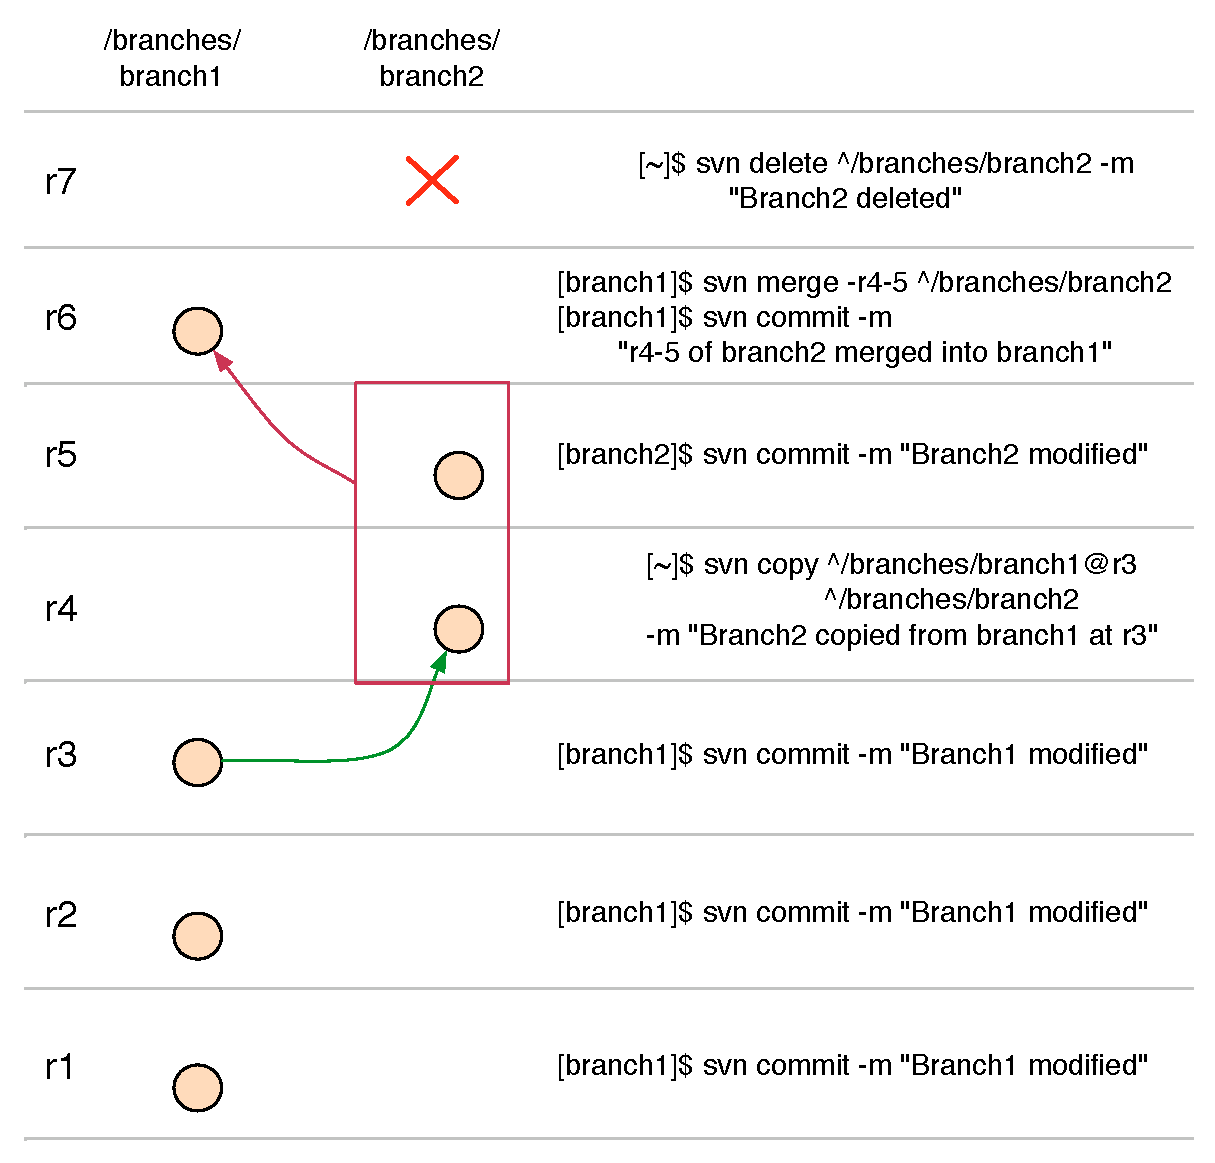
\includegraphics[width=\textwidth]{img/legend/svn_layer.pdf}%
\captionof{figure}{Subversion history layer.}
\label{svn_layer}%
\end{center}

2. Git history layer. See diagram \ref{git_layer}.
\begin{center}
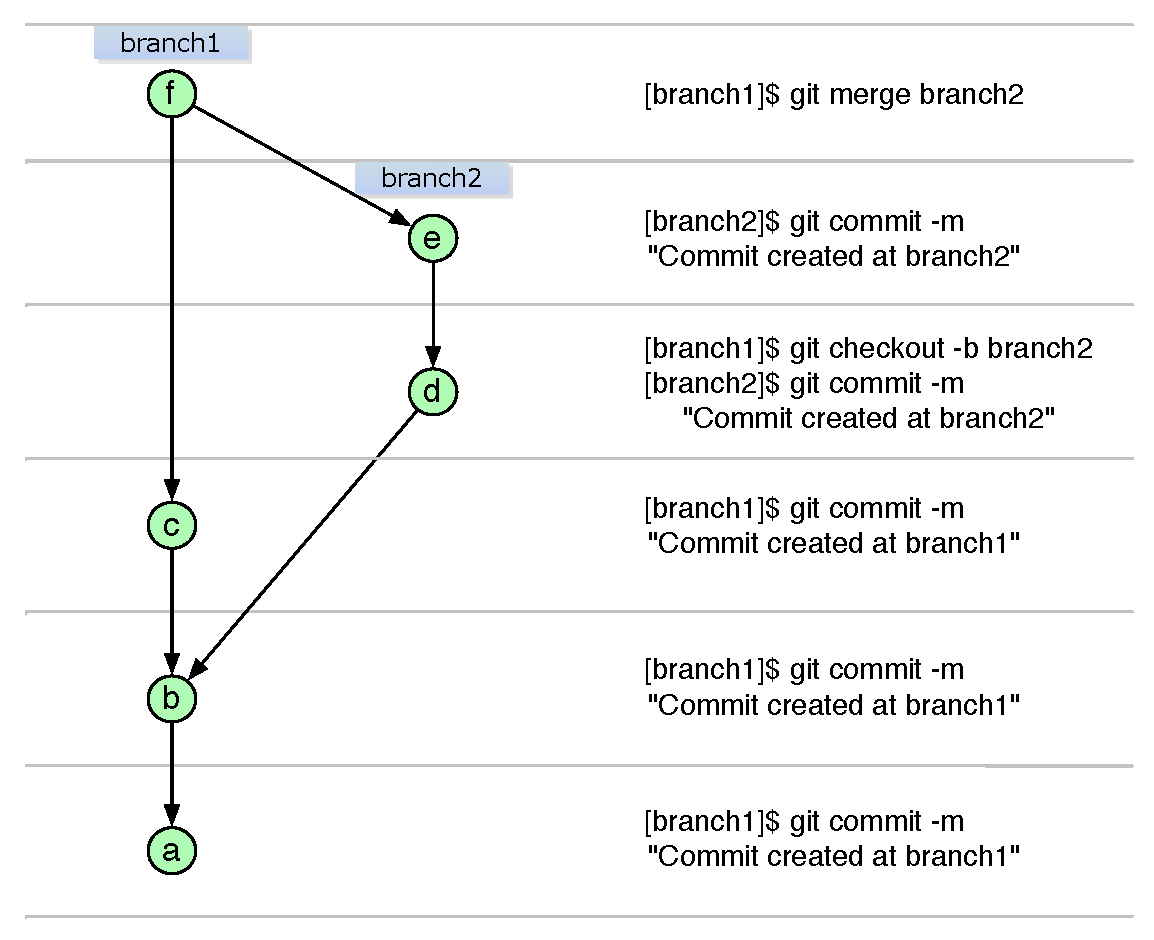
\includegraphics[width=\textwidth]{img/legend/git_layer.pdf}%
\captionof{figure}{Git history layer.}
\label{git_layer}%
\end{center}

First parent of merge commits will be always depicted as vertical arrow.
\\\\
To illustrate combined history we join described layers to put Git commits on top of corresponding SVN revisions as depicted at diagram \ref{both_layers}.
\begin{center}
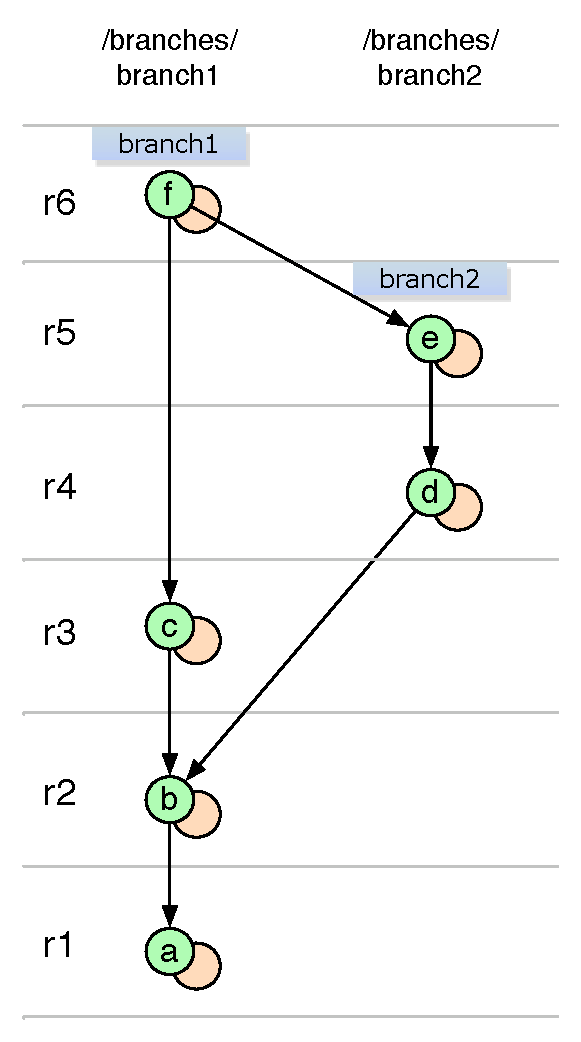
\includegraphics[width=7.0cm]{img/legend/generalized_history.pdf}%
\captionof{figure}{Combined history.}
\label{both_layers}%
\end{center}